\section{Background}
\label{sec.preliminary}
\begin{sloppypar}


\begin{figure}[t]
 \vspace{-3mm}
     \centering
     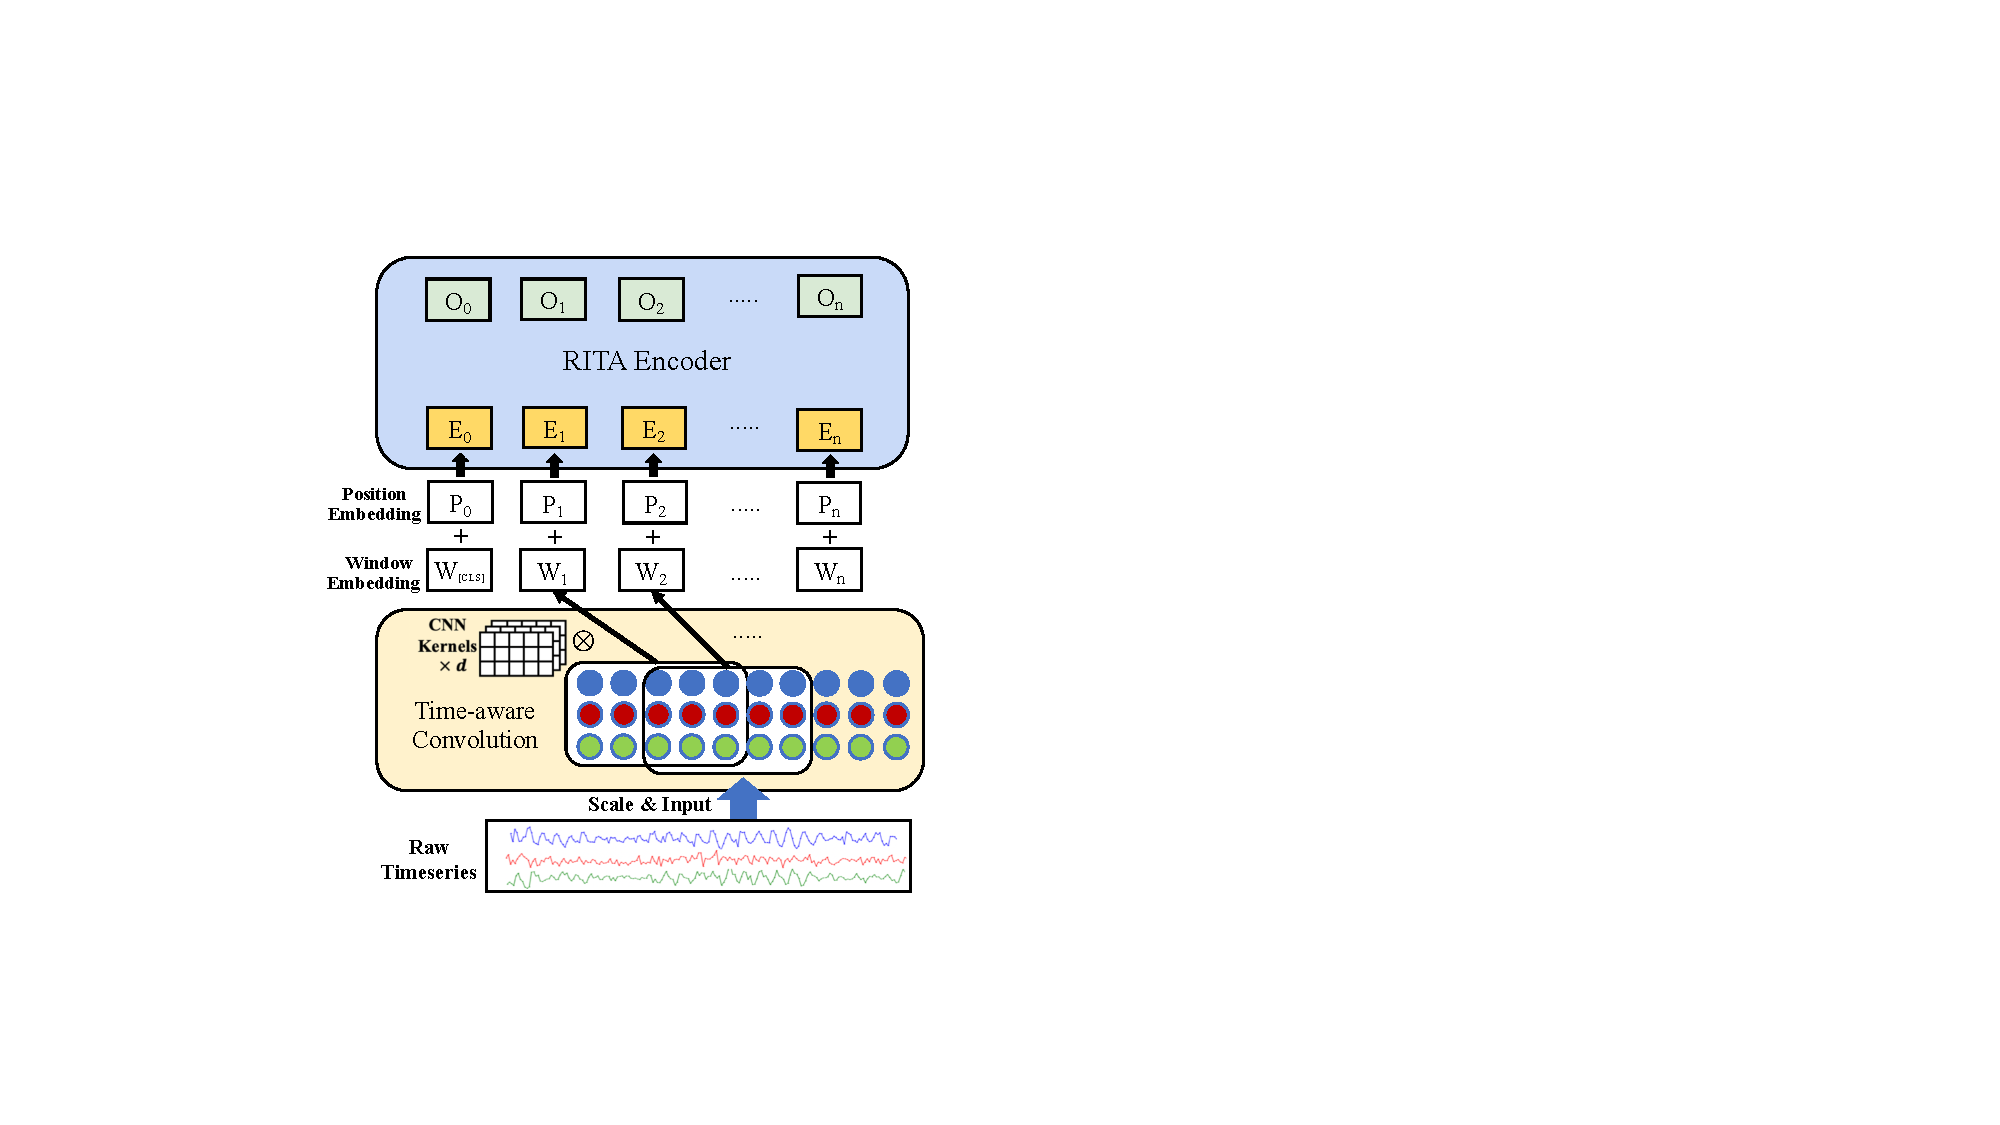
\includegraphics[width=0.8\columnwidth]{figures/model_arch.pdf}
     \vspace{-2mm}
     \caption{\system Architecture}
     \label{fig.convolution}
     \vspace{-4mm}
\end{figure}


% \begin{figure}[t]
% \vspace{-2mm}
%     \centering
%     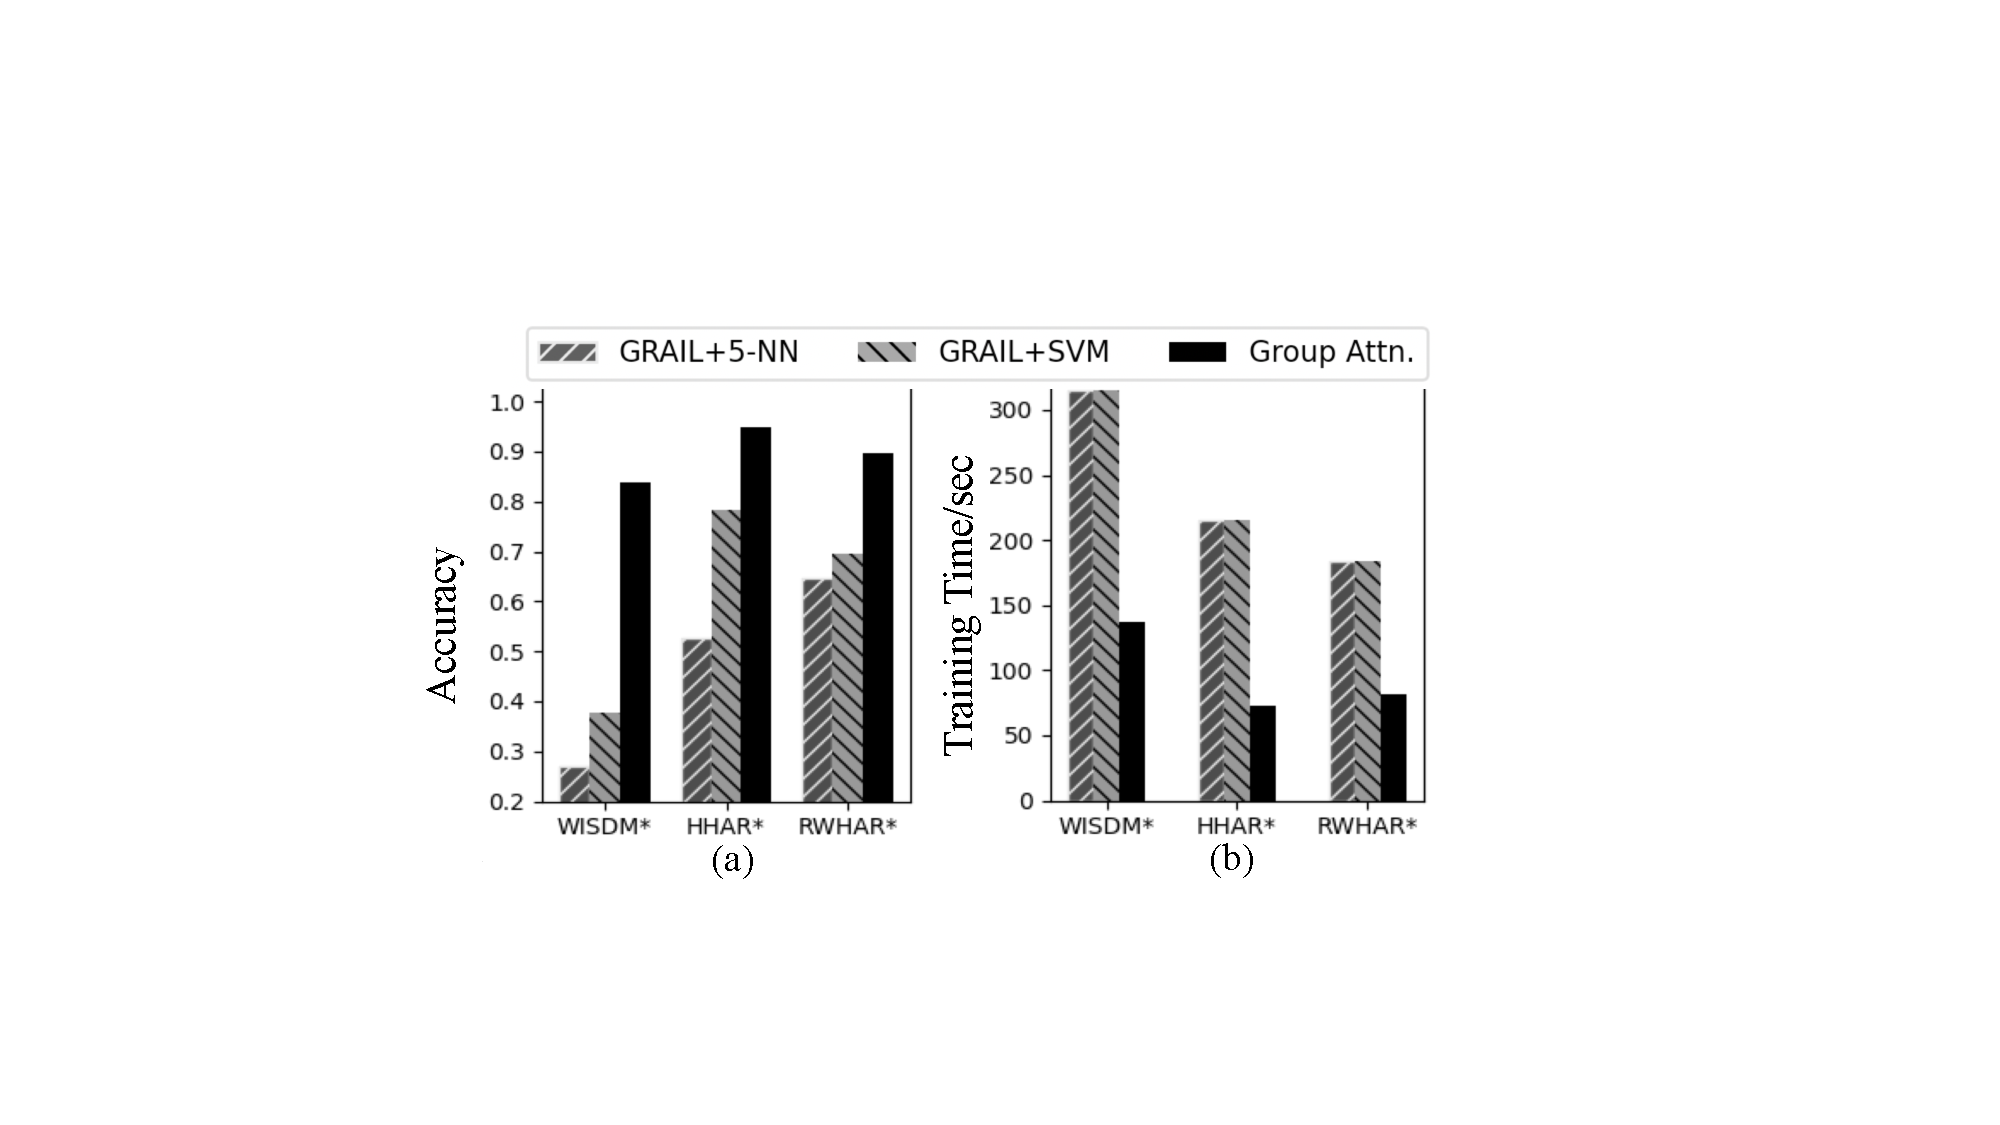
\includegraphics[width=0.8\columnwidth]{figures/uni_bar.pdf}
%     \vspace{-4mm}
% %    \setcaptionwidth{3.5in}
%     \caption{Comparison to non-deep learning method (uni-variate data).}
%     %Metric is given in accuracy on classification. Efficiency is measured by the average training time per epoch. \jm{revised}}
%     \label{fig.full_uni}
%     \vspace{-5mm}
% \end{figure}

We provide some background on the canonical self-attention module in the Transformer\cite{DBLP:conf/nips/VaswaniSPUJGKP17}.
A \emph{self-attention} module takes $n$ hidden embedding vectors $H \in \mathbb{R}^{n*d_h}$ as input, then projects them to queries ($Q$), keys ($K$) and values ($V$) and performs Scaled-dot Product Attention, which given input hidden state $H$, is computed by:

\vspace{-0.5mm}
\begin{equation}
\label{eq.attention}
\small
\begin{aligned}
    Q = HW_Q, K = HW_K, V = HW_V \\
    O = AV = SoftMax(\frac{QK^T}{\sqrt{d_k}})V 
\end{aligned}
\end{equation}
\vspace{-1mm}
Where $W_Q \in \mathbb{R}^{d_h*d_k}, W_K \in \mathbb{R}^{d_h*d_k}, W_V \in \mathbb{R}^{d_h*d_v}$ are projection matrices for generating $Q,K,V$.
$Q\in \mathbb{R}^{n*d_k}$ is also regarded as the packing of $n$ query vectors $\{q_1,...,q_n\}$ with dimension $d_k$ into a matrix. $K \in \mathbb{R}^{n*d_k}, V\in \mathbb{R}^{n*d_v}$ are regarded as the packing of key vectors $\{k_1,...,k_n\}$ and value vectors $\{v_1,...,v_n\}$ in the same way.

Given a matrix $M \in \mathbb{R}^{L*n}$, the softmax function normalizes $M$ to ensure the sum of each row equals to 1, as shown below.
\vspace{-2mm}
\begin{equation}
\label{eq.softmax}
SoftMax(M_{i,j})=\frac{exp(M_{i,j})}{\sum_{k=0}^{n-1} exp(M_{i,k})}\\
\end{equation}

Note the attention matrix A is an $n \times n$ matrix, where $n$ represents the number of elements in the input sequence (e.g. words in NLP).

% \noindent\textbf{GPU Memory Bottleneck.} Note the attention matrix A is an $n \times n$ matrix, where $n$ represents the number of elements in the input sequence (e.g. words in NLP). 
% Because GPUs have limited memory, self-attention is not scalable to long sequence due to its quadratic space complexity. 

\end{sloppypar}

% \zi{This brief section seems to slightly be background, slightly motivation or constraints or problem statement. Maybe we can be clearer in what we want to communicate? (1) It looks like perhaps we are reviewing self-attention? (2) Are we trying to motivate the problems we solve, as well, with the mention of the GPU memory bottleneck? At minimum I think we need a bridge statement: we will try to do attention, taking into account the constraints of GPU memory to go below nxn, or something.}